\pdfminorversion=4
\documentclass[first=red,second=purple,logo=yellowexc]{aaltoslides}
%\documentclass{aaltoslides} % DEFAULT
%\documentclass[first=purple,second=lgreen,logo=redque,normaltitle,nofoot]{aaltoslides} % SOME OPTION EXAMPLES
\usepackage{listings}
\usepackage{booktabs}
\lstdefinelanguage{JavaScript}{
  keywords={typeof, new, true, false, catch, function, return, null, catch, switch, var, if, in, while, do, else, case, break},
  keywordstyle=\color{blue}\bfseries,
  ndkeywords={class, export, boolean, throw, implements, import, this},
  ndkeywordstyle=\color{darkgray}\bfseries,
  identifierstyle=\color{black},
  sensitive=false,
  comment=[l]{//},
  morecomment=[s]{/*}{*/},
  commentstyle=\color{purple}\ttfamily,
  stringstyle=\color{red}\ttfamily,
  morestring=[b]',
  morestring=[b]"
}
\lstset{frame=tb,
  language=JavaScript,
  aboveskip=3mm,
  belowskip=3mm,
  showstringspaces=false,
  columns=flexible,
  basicstyle={\small\ttfamily},
  numbers=none,
  numberstyle=\tiny\color{gray},
  keywordstyle=\color{blue},
  commentstyle=\color{dkgreen},
  stringstyle=\color{mauve},
  breaklines=true,
  breakatwhitespace=true
  tabsize=3
}
\usepackage[latin9]{inputenc}
\usepackage[T1]{fontenc}
\usepackage{graphicx}
\usepackage{amssymb,amsmath}
\usepackage{url}
\usepackage{lastpage}
\usepackage{caption}
\usepackage{subcaption}

\title{Performance analysis of topologies for Web-based Real-Time Communication}

\author[Albert Abello Lozano]{Albert Abello Lozano}
\institute[COMNET]{Supervisor: J\"{o}rg Ott\\Instructor: Varun Singh\\Communication and Networking Department\\
Aalto University, School of Science and Technology\\albert.abello.lozano@aalto.fi}

\aaltofootertext{Performance analysis of topologies for WebRTC}{May 22, 2013}{\arabic{page}/\pageref{LastPage}\ }

\date{Espoo , May 22, 2013}

\begin{document}

%%%%%%%%%%%%%%%%%%%%%%%%%%%%%%%%%%%%%%%%%%%%%%%%%%%%%%%%%%%%%%%%%%%%%%%%%%%%%%%%%%%%%%%%%%%%%

\aaltotitleframe

%%%%%%%%%%%%%%%%%%%%%%%%%%%%%%%%%%%%%%%%%%%%%%%%%%%%%%%%%%%%%%%%%%%%%%%%%%%%%%%%%%%%%%%%%%%%%

\begin{frame}{Outline}
\begin{itemize}
\item Background
\item WebRTC
\item Topologies
%\item Metrics
\item Evaluation environment
\item Tests and results
\item Conclusions
\end{itemize}
\end{frame}

%%%%%%%%%%%%%%%%%%%%%%%%%%%%%%%%%%%%%%%%%%%%%%%%%%%%%%%%%%%%%%%%%%%%%%%%%%%%%%%%%%%%%%%%%%%%%

%\begin{frame}{Introduction}
%
%\begin{itemize}
%\item Need of connectivity between people
%\item Real-time communication is in our daily life
%\item Complex interactive web applications are everywhere 
%\item Developers need a way to handle real-time cross-interoperable apps in the web
%\end{itemize}
%
%%\begin{block}
%%\alert{WebRTC}
%%\end{block}
%\begin{figure}[h]
%  \centering
%  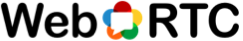
\includegraphics[width=5cm]{customLogo}
%\end{figure}
%\end{frame}

%%%%%%%%%%%%%%%%%%%%%%%%%%%%%%%%%%%%%%%%%%%%%%%%%%%%%%%%%%%%%%%%%%%%%%%%%%%%%%%%%%%%%%%%%%%%%

\begin{frame}{Background}

\begin{itemize}
\item Open sourced by Google
\item First introduced in May 2011
\item Designed in conjunction by the IETF and W3C
\item Still in ongoing discussion
\item Works using high level JavaScript APIs 
\item First version to be delivered by Q4 2013
\item Uses existing technologies derived from SIP
\end{itemize}
\end{frame}

%%%%%%%%%%%%%%%%%%%%%%%%%%%%%%%%%%%%%%%%%%%%%%%%%%%%%%%%%%%%%%%%%%%%%%%%%%%%%%%%%%%%%%%%%%%%%
\begin{frame}{Support}

Browser vendors that are actively supporting WebRTC:
\begin{itemize}
\item Google
\item Mozilla Foundation
\item Opera
\item Microsoft (separate spec)
\end{itemize}
Equipment and service providers involved:
\begin{itemize}
\item Ericsson
\item Cisco
\end{itemize}
\end{frame}
%%%%%%%%%%%%%%%%%%%%%%%%%%%%%%%%%%%%%%%%%%%%%%%%%%%%%%%%%%%%%%%%%%%%%%%%%%%%%%%%%%%%%%%%%%%%%

%\begin{frame}{Support}
%
\includegraphics[width=3cm]{Google-eps-converted-to.pdf}\hspace{10pt}
%
\includegraphics[width=3cm]{Opera-eps-converted-to.pdf}\hspace{10pt}
%
\includegraphics[width=3cm]{Mozilla_Firefox-eps-converted-to.pdf}\\[0.2cm]
%
\includegraphics[trim=0cm 5cm 0cm 0cm, clip=true, width=3cm]{cisco-logo-eps-converted-to.pdf}\hspace{10pt}
%
\includegraphics[width=3cm]{Internet_Explorer_4-eps-converted-to.pdf}\hspace{10pt}
%
\includegraphics[trim=9cm 9cm 9cm 9cm, clip=true,width=3cm]{ericsson_logo-eps-converted-to.pdf}\\[0.2cm]
%
%\end{frame}
%%%%%%%%%%%%%%%%%%%%%%%%%%%%%%%%%%%%%%%%%%%%%%%%%%%%%%%%%%%%%%%%%%%%%%%%%%%%%%%%%%%%%%%%%%%%%

\begin{frame}{WebRTC}

\begin{itemize}
\item Provides real-time peer-to-peer media and data transport using browsers
\item {\color{red}Plugin-free}, mechanisms are integrated on the browsers
\item Interoperable between vendors
\item Uses JavaScript APIs to enable the features
\item Federated domain video calls
%\item Combines two high-level JavaScript APIs:
%\begin{itemize}
%\item {\it GetUserMedia()}
%\item {\it PeerConnection()}
%\end{itemize}
%\item Uses different specific objects:
%\begin{itemize}
%\item {\it MediaSream}
%\item {\it MediaStreamTrack}
%\item {\it DataChannel}
%\end{itemize}
\item {\it Google Chrome} and {\it Mozilla Firefox} implement all the APIs
\item {\it Opera} only includes {\it GetUserMedia}
\end{itemize}
\end{frame}

%%%%%%%%%%%%%%%%%%%%%%%%%%%%%%%%%%%%%%%%%%%%%%%%%%%%%%%%%%%%%%%%%%%%%%%%%%%%%%%%%%%%%%%%%%%%%

%\begin{frame}{WebRTC network internals}
%\begin{itemize}
%\item RTP and RTCP multiplexed over the same port
%\item SDP for signaling content
%\item SCTP and DTLS for secure data
%\item SRTP for media
%\item STUN, TURN and ICE for NAT reversal
%\item {\color{blue}All traffic over UDP}
%\end{itemize}
%\end{frame}

%%%%%%%%%%%%%%%%%%%%%%%%%%%%%%%%%%%%%%%%%%%%%%%%%%%%%%%%%%%%%%%%%%%%%%%%%%%%%%%%%%%%%%%%%%%%%

\begin{frame}{WebRTC protocol stack}

\begin{figure}[h]
  \centering
  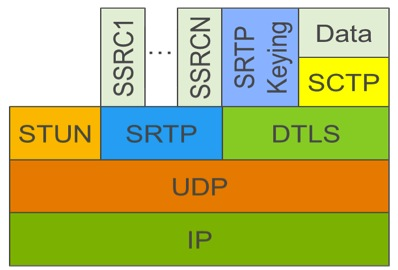
\includegraphics[width=1\textwidth]{protocolStack.pdf}
\end{figure}

\end{frame}

%%%%%%%%%%%%%%%%%%%%%%%%%%%%%%%%%%%%%%%%%%%%%%%%%%%%%%%%%%%%%%%%%%%%%%%%%%%%%%%%%%%%%%%%%%%%%
\begin{frame}{WebRTC implementation}

\begin{itemize}
\item VP8 and H.264 video codec
\item G711 and Opus as audio codec
%\item H.264 video codec in some browser vendors
\item {\color{blue} JSEP} is the protocol between the application and the browser
\end{itemize}
\alert{Media codecs are still on an ongoing discussion}
\end{frame}

%%%%%%%%%%%%%%%%%%%%%%%%%%%%%%%%%%%%%%%%%%%%%%%%%%%%%%%%%%%%%%%%%%%%%%%%%%%%%%%%%%%%%%%%%%%%%

\begin{frame}{JSEP signaling model}

\begin{figure}[h]
  \centering
  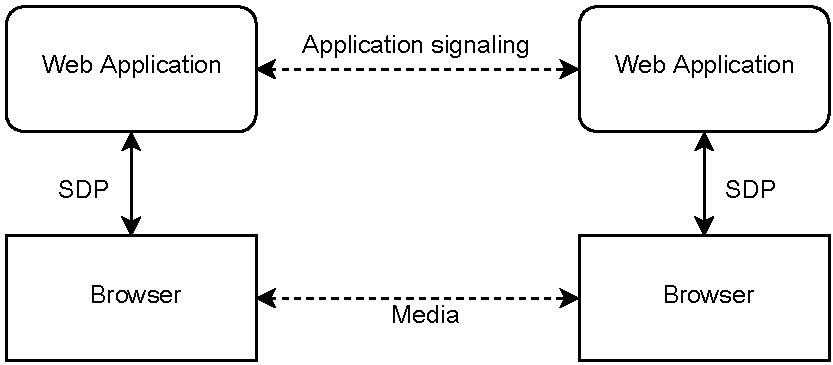
\includegraphics[width=1\textwidth]{JSEP.pdf}
\end{figure}

\end{frame}
%%%%%%%%%%%%%%%%%%%%%%%%%%%%%%%%%%%%%%%%%%%%%%%%%%%%%%%%%%%%%%%%%%%%%%%%%%%%%%%%%%%%%%%%%%%%%

\begin{frame}{WebRTC APIs}

\begin{itemize}
\item Combines two high-level JavaScript APIs:
\begin{itemize}
\item {\it GetUserMedia()}
\item {\it PeerConnection()}
\end{itemize}
\item Uses different specific objects:
\begin{itemize}
\item {\it MediaSream}
\item {\it MediaStreamTrack}
\item {\it DataChannel}
\end{itemize}
\item Control and monitoring:
\begin{itemize}
\item {\it getStats()} method is used for monitoring
\item JSON objects change the constraints for video and networking
\end{itemize}
\item {\it Google Chrome} and {\it Mozilla Firefox} implement all the APIs
\item {\it Opera} only includes {\it GetUserMedia}
\end{itemize}
\end{frame}

%%%%%%%%%%%%%%%%%%%%%%%%%%%%%%%%%%%%%%%%%%%%%%%%%%%%%%%%%%%%%%%%%%%%%%%%%%%%%%%%%%%%%%%%%%%%%

\begin{frame}[fragile]{{\it GetUserMedia()}}

Provides access to media devices and returns a {\it MediaStream} object.

\lstset{language=JavaScript}
\begin{lstlisting}
navigator.webkitGetUserMedia(cameraConstraints(), gotStream, function() {
   console.log("GetUserMedia failed");
});
    
function gotStream(stream) {
   //Stream is the MediaStream object returned by the API and played in HTML local-video element
   console.log("GetUserMedia succeeded");
   document.getElementById("local-video").src = webkitURL.createObjectURL(stream);
}
\end{lstlisting}

\end{frame}

%%%%%%%%%%%%%%%%%%%%%%%%%%%%%%%%%%%%%%%%%%%%%%%%%%%%%%%%%%%%%%%%%%%%%%%%%%%%%%%%%%%%%%%%%%%%%
\begin{frame}[fragile]{{\it MediaStream} and {\it MediaStreamTrack}}

\begin{figure}[h]
  \centering
  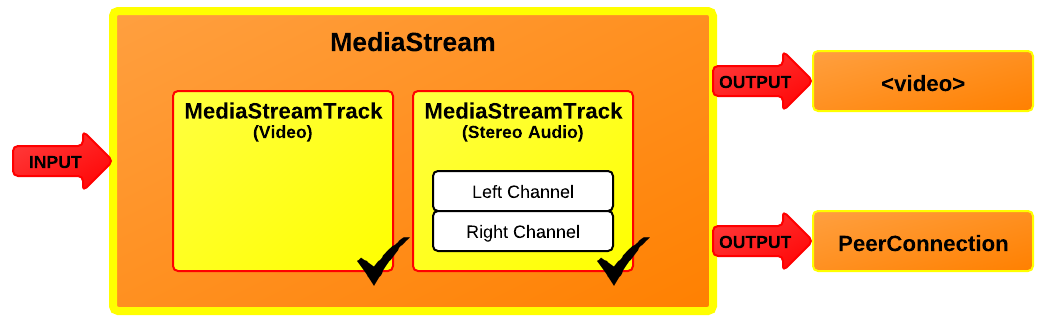
\includegraphics[width=1\textwidth]{mediastreamAPI.png}
\end{figure}

\end{frame}

%%%%%%%%%%%%%%%%%%%%%%%%%%%%%%%%%%%%%%%%%%%%%%%%%%%%%%%%%%%%%%%%%%%%%%%%%%%%%%%%%%%%%%%%%%%%%

\begin{frame}[fragile]{{\it PeerConnection()}}

Builds a point-to-point connection
\lstset{language=JavaScript}
\begin{lstlisting}
pc = new webkitRTCPeerConnection(pc_config);
pc.onicecandidate = iceCallback;
pc.addStream(localstream);
function iceCallback(event){
   if (event.candidate) {
      sendMessage(event.candidate);
   }
}
pc.addIceCandidate(new RTCIceCandidate(event.candidate));
pc.onaddstream = gotRemoteStream; 
function gotRemoteStream(e){
   document.getElementById("remote-video").src = URL.createObjectURL(e.stream);
}
\end{lstlisting}

\end{frame}

%%%%%%%%%%%%%%%%%%%%%%%%%%%%%%%%%%%%%%%%%%%%%%%%%%%%%%%%%%%%%%%%%%%%%%%%%%%%%%%%%%%%%%%%%%%%%

%\begin{frame}{Security in WebRTC}
%
%JavaScript libraries can provide cross-scripting and trust vulnerabilities
%\begin{figure}[h]
%  \centering
%  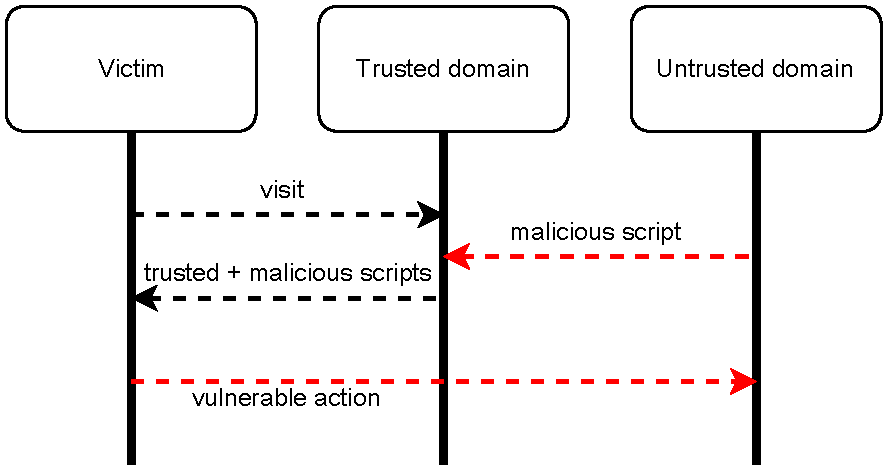
\includegraphics[width=1\textwidth]{xss.pdf}
%\end{figure}
%\end{frame}
%%%%%%%%%%%%%%%%%%%%%%%%%%%%%%%%%%%%%%%%%%%%%%%%%%%%%%%%%%%%%%%%%%%%%%%%%%%%%%%%%%%%%%%%%%%%%

\begin{frame}{Topologies}

Possible topologies for real-time communication:
\begin{itemize}
\item Point-to-Point
\item One-to-Many
\item Many-to-Many
\item MCU
\item Overlay
\begin{itemize}
\item Spoke-hub
\item Tree
\end{itemize}
\end{itemize}
\end{frame}

%%%%%%%%%%%%%%%%%%%%%%%%%%%%%%%%%%%%%%%%%%%%%%%%%%%%%%%%%%%%%%%%%%%%%%%%%%%%%%%%%%%%%%%%%%%%%
\begin{frame}{Point-to-Point}

\begin{figure}[h]
  \centering
  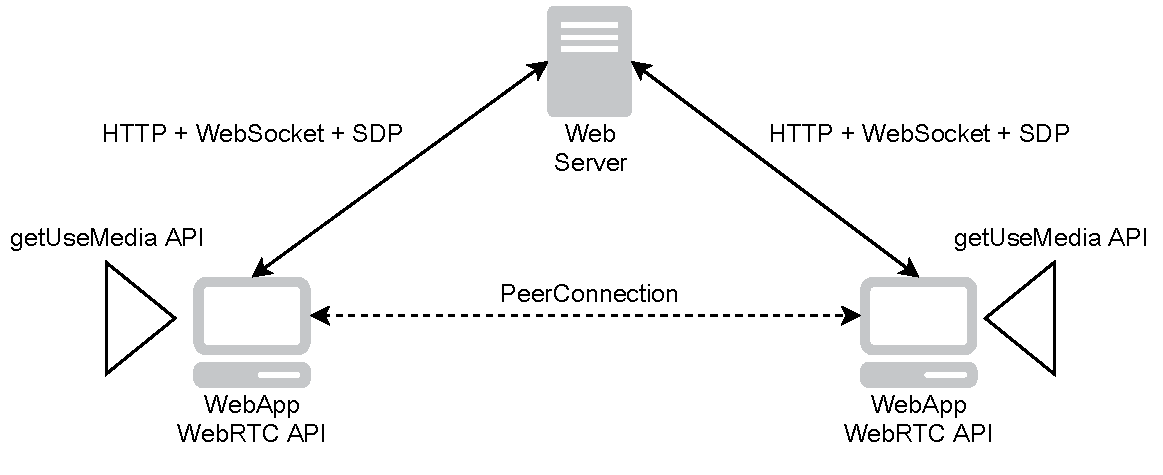
\includegraphics[width=1\textwidth]{webrtcExample.pdf}
\end{figure}
\end{frame}

%%%%%%%%%%%%%%%%%%%%%%%%%%%%%%%%%%%%%%%%%%%%%%%%%%%%%%%%%%%%%%%%%%%%%%%%%%%%%%%%%%%%%%%%%%%%%
\begin{frame}{Topologies}

\begin{figure}[h]
        \centering
        \begin{subfigure}[b]{0.3\textwidth}
                \centering
                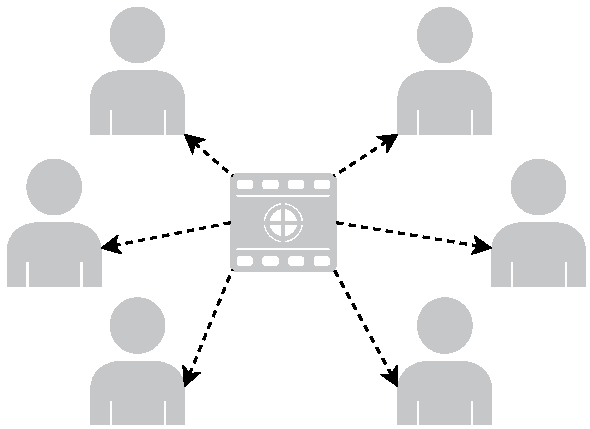
\includegraphics[width=\textwidth]{star.pdf}
                \caption{One-to-Many}
        \end{subfigure}%
        ~ %add desired spacing between images, e. g. ~, \quad, \qquad etc.
          %(or a blank line to force the subfigure onto a new line)
        \begin{subfigure}[b]{0.3\textwidth}
                \centering
                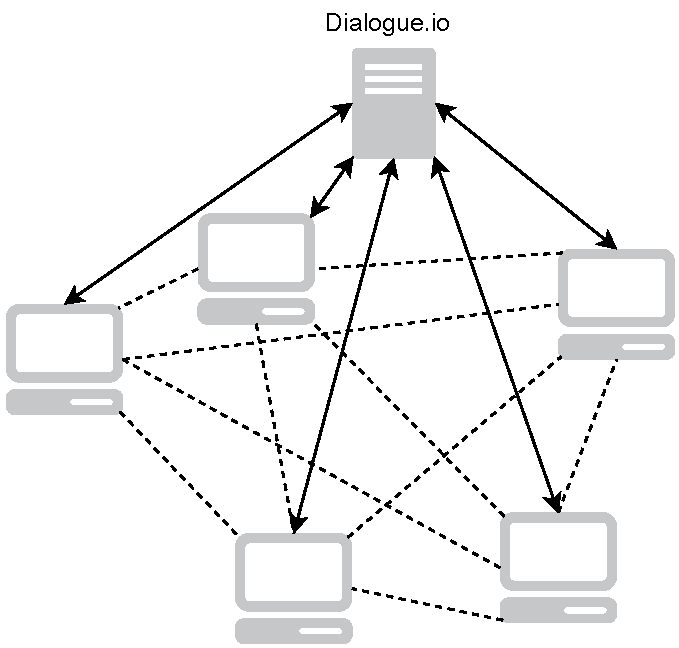
\includegraphics[width=\textwidth]{mesh.pdf}
                 \caption{Many-to-Many}
        \end{subfigure}
        \begin{subfigure}[b]{0.3\textwidth}
                \centering
                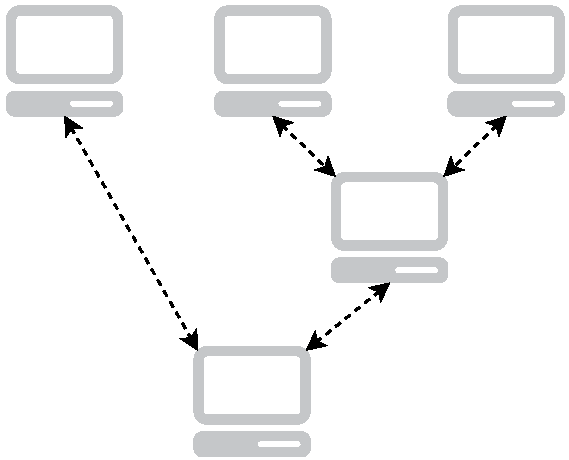
\includegraphics[width=\textwidth]{three.pdf}
                \caption{Tree}
        \end{subfigure}%
        ~ %add desired spacing between images, e. g. ~, \quad, \qquad etc.
          %(or a blank line to force the subfigure onto a new line)
        \begin{subfigure}[b]{0.3\textwidth}
                \centering
                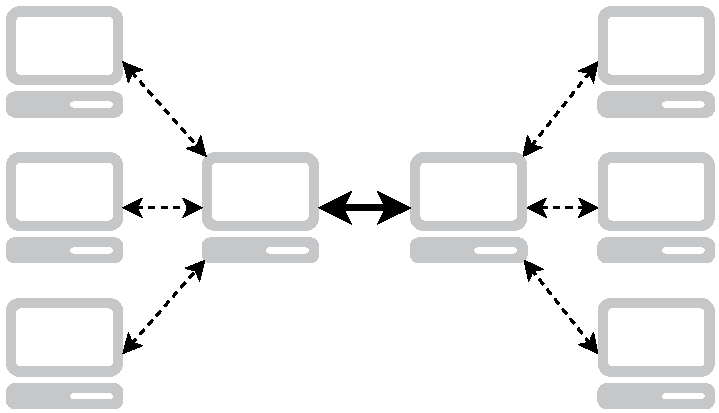
\includegraphics[width=\textwidth]{hubandspoke.pdf}
                 \caption{Spoke-Hub}
        \end{subfigure}
\end{figure}
\end{frame}

%%%%%%%%%%%%%%%%%%%%%%%%%%%%%%%%%%%%%%%%%%%%%%%%%%%%%%%%%%%%%%%%%%%%%%%%%%%%%%%%%%%%%%%%%%%%%
%\begin{frame}{Overlay}
%
%\begin{figure}[h]
%        \centering
%        \begin{subfigure}[b]{0.5\textwidth}
%                \centering
%                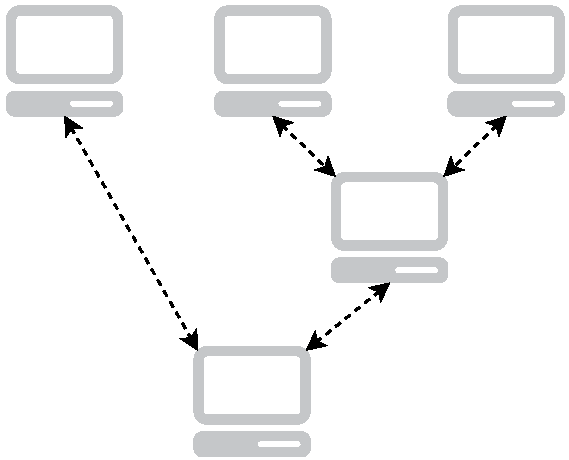
\includegraphics[width=\textwidth]{three.pdf}
%                \caption{Tree}
%        \end{subfigure}%
%        ~ %add desired spacing between images, e. g. ~, \quad, \qquad etc.
%          %(or a blank line to force the subfigure onto a new line)
%        \begin{subfigure}[b]{0.5\textwidth}
%                \centering
%                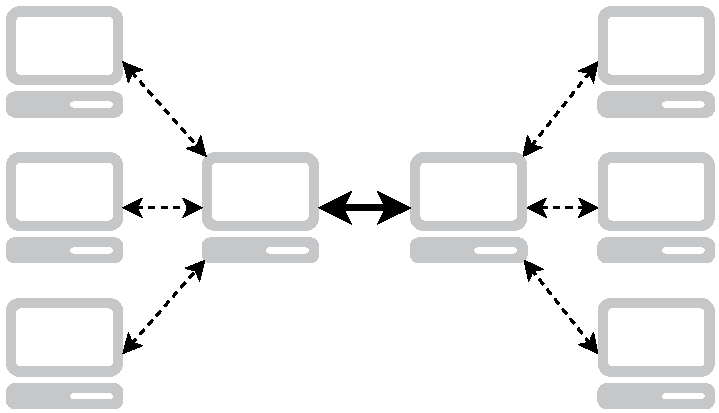
\includegraphics[width=\textwidth]{hubandspoke.pdf}
%                 \caption{Spoke-Hub}
%        \end{subfigure}
%\end{figure}
%\end{frame}

%%%%%%%%%%%%%%%%%%%%%%%%%%%%%%%%%%%%%%%%%%%%%%%%%%%%%%%%%%%%%%%%%%%%%%%%%%%%%%%%%%%%%%%%%%%%%

\begin{frame}{Performance Metrics}

%\begin{itemize}
Network:
\begin{itemize}
\item Packet loss
\item Round-Trip Time and One-Way Delay
\item Throughput
\item Inter-Arrival Time and Jitter
\end{itemize}

Host:
\begin{itemize}
\item Resources
\item Setup time
\item Call failure rate
\item Encoding and decoding
\end{itemize}

%\end{itemize}

\end{frame}
%%%%%%%%%%%%%%%%%%%%%%%%%%%%%%%%%%%%%%%%%%%%%%%%%%%%%%%%%%%%%%%%%%%%%%%%%%%%%%%%%%%%%%%%%%%%%
%\begin{frame}{Tools used}
%
%Client:
%\begin{itemize}
%\item Google Chrome
%\item Connection Monitor (ConMon)
%\item Statistics API (Stats API)
%\item Fake video device for Chrome
%\end{itemize}
%Server:
%\begin{itemize}
%\item Restund
%\item Dummynet
%\item Application server (Node.js)
%\end{itemize}
%
%\end{frame}

%%%%%%%%%%%%%%%%%%%%%%%%%%%%%%%%%%%%%%%%%%%%%%%%%%%%%%%%%%%%%%%%%%%%%%%%%%%%%%%%%%%%%%%%%%%%%
\begin{frame}{Evaluation Environment}

\begin{figure}[h]
  \centering
  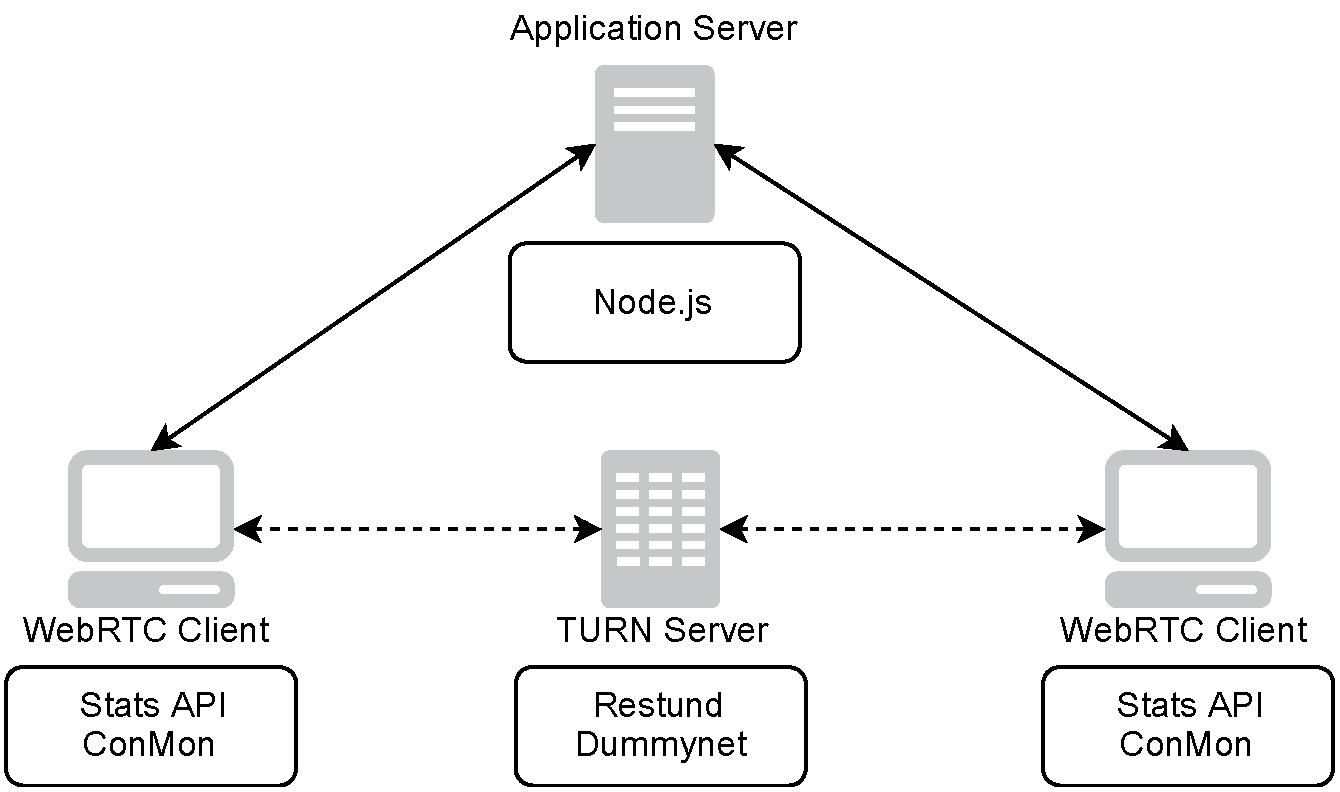
\includegraphics[width=1\textwidth]{evaluation_arch.pdf}
\end{figure}
\end{frame}

%%%%%%%%%%%%%%%%%%%%%%%%%%%%%%%%%%%%%%%%%%%%%%%%%%%%%%%%%%%%%%%%%%%%%%%%%%%%%%%%%%%%%%%%%%%%%

\begin{frame}{ConMon vs StatsAPI}
\begin{itemize}
\item Incoming stream
\end{itemize}
\begin{figure}[h]
  \centering
  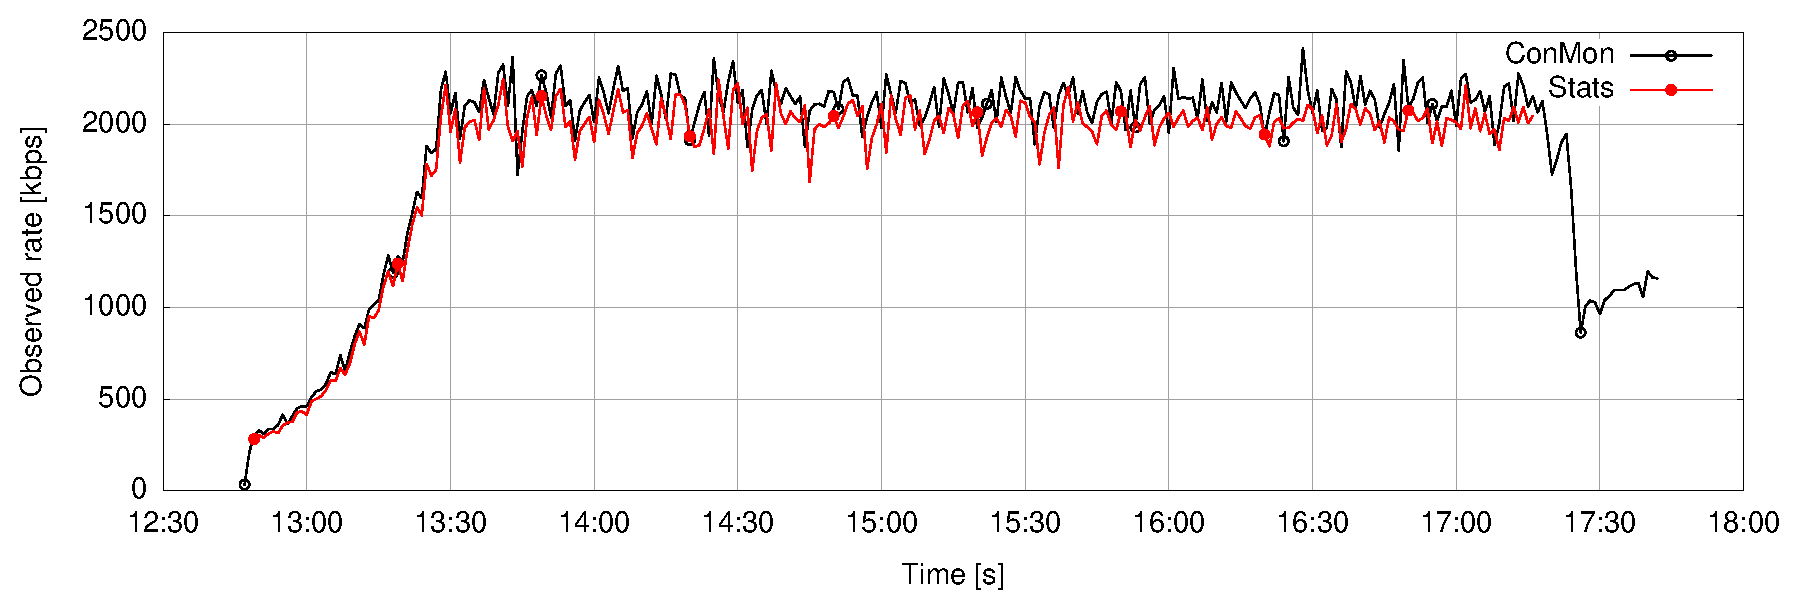
\includegraphics[width=0.75\textwidth]{p2p_incomming_cable_sample.pdf}
  %\caption{Incoming stream}
\end{figure}
\begin{itemize}
\item Outgoing stream
\end{itemize}
\begin{figure}[h]
  \centering
  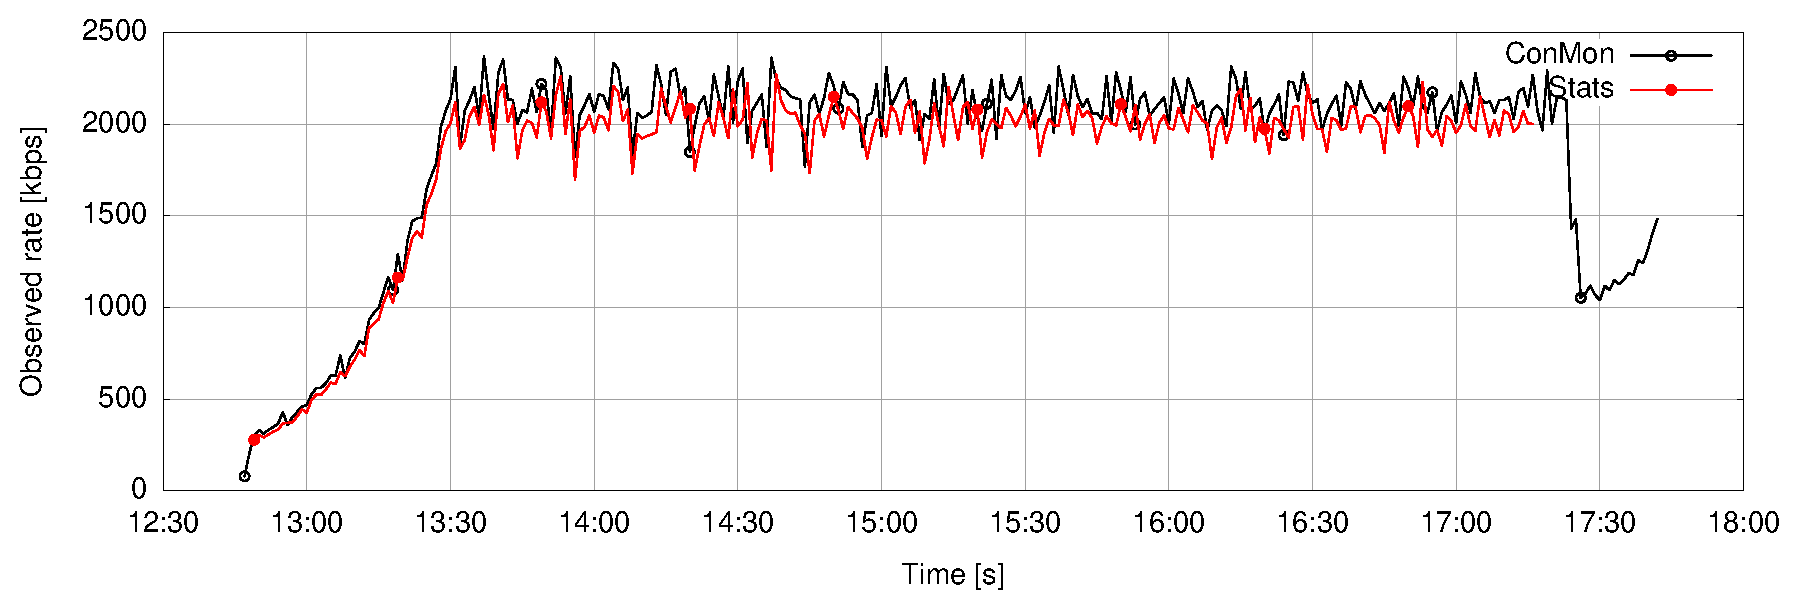
\includegraphics[width=0.75\textwidth]{p2p_outgoing_cable_sample.pdf}
  %\caption{Outgoing stream}
\end{figure}
%\begin{figure}[h]
%        \centering
%        \begin{subfigure}[b]{0.5\textwidth}
%                \centering
%                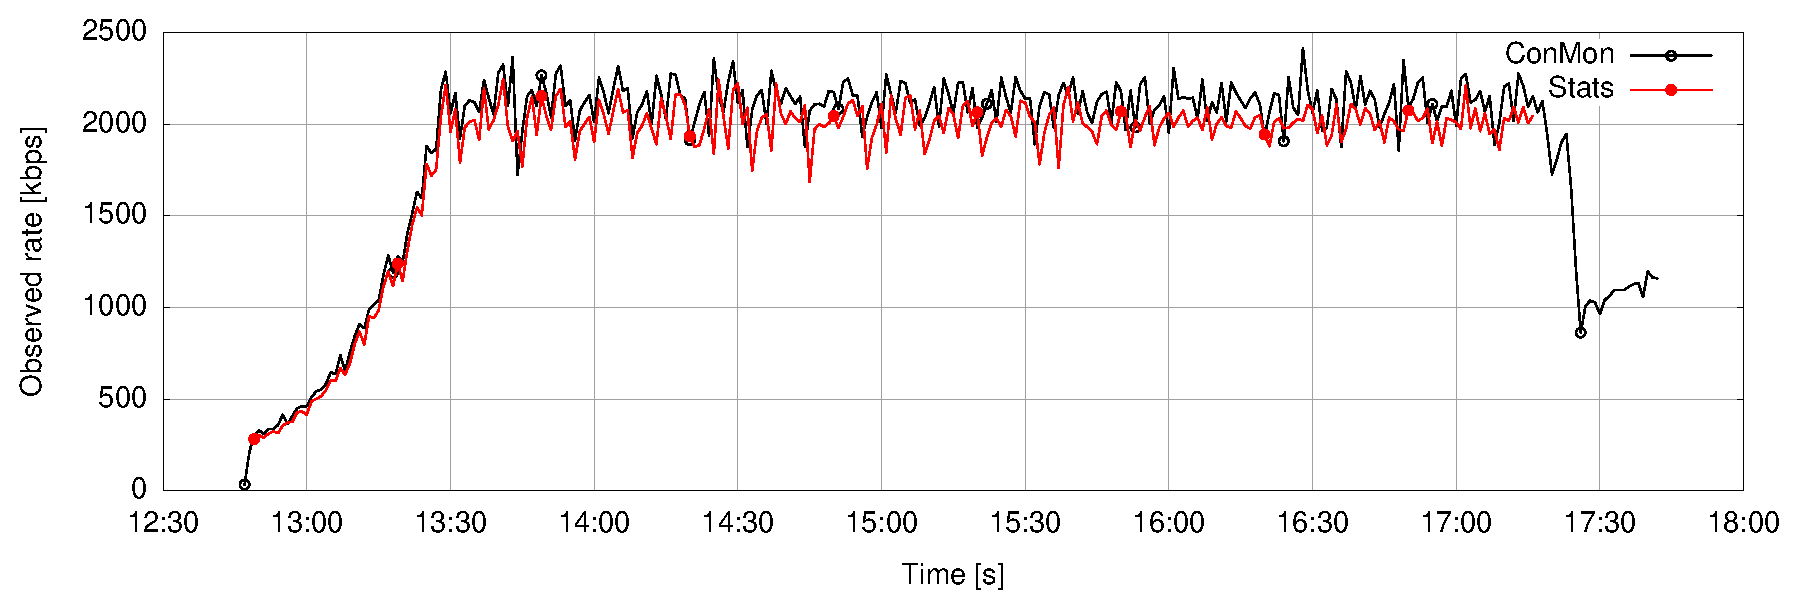
\includegraphics[width=\textwidth]{p2p_incomming_cable_sample.pdf}
%                \caption{Incoming stream}
%        \end{subfigure}%
%        ~ %add desired spacing between images, e. g. ~, \quad, \qquad etc.
%          %(or a blank line to force the subfigure onto a new line)
%        \begin{subfigure}[b]{0.5\textwidth}
%                \centering
%                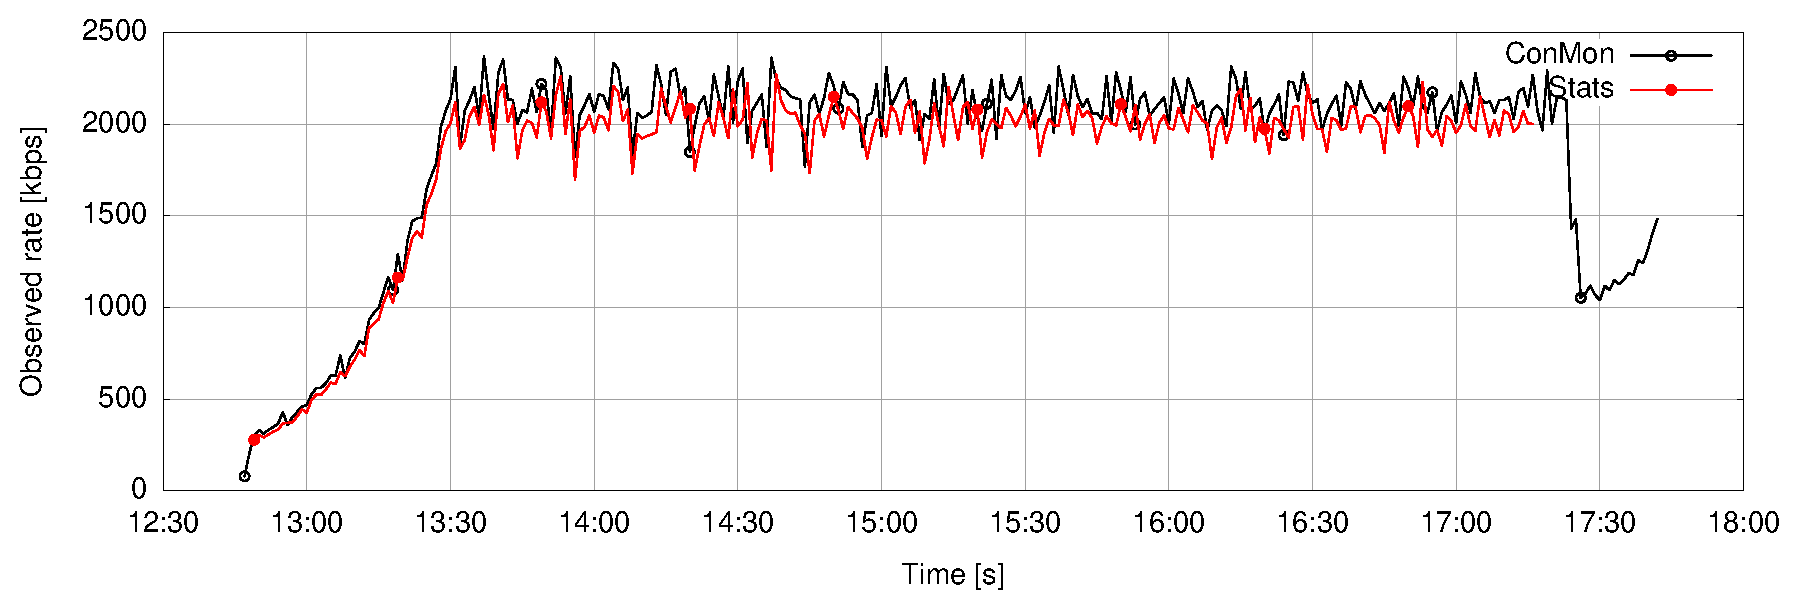
\includegraphics[width=\textwidth]{p2p_outgoing_cable_sample.pdf}
%                 \caption{Outgoing stream}
%        \end{subfigure}
%\end{figure}
\end{frame}

%%%%%%%%%%%%%%%%%%%%%%%%%%%%%%%%%%%%%%%%%%%%%%%%%%%%%%%%%%%%%%%%%%%%%%%%%%%%%%%%%%%%%%%%%%%%%
%
%\begin{frame}{Congestion mechanisms in WebRTC}
%
%\begin{itemize}
%\item UDP has difficulties for rate adaption 
%\item Sender and Receiver RTCP reports used for rate adjustment
%\item Receiver Estimated Maximum Bitrate (REMB) extension for RTCP
%\item Utilizes specific {\color{red}Google algorithm} for rate adaption based on packet loss
%\begin{itemize}
%\item Under 2\% increases rate
%\item 2-10\% reminds unchanged
%\item +10\% adapts rate based on packet loss ratio
%\end{itemize}
%\item Rate limit by the TCP Friendly Rate Control (TFRC) formula
%\end{itemize}
%\end{frame}
%%%%%%%%%%%%%%%%%%%%%%%%%%%%%%%%%%%%%%%%%%%%%%%%%%%%%%%%%%%%%%%%%%%%%%%%%%%%%%%%%%%%%%%%%%%%%

\begin{frame}{Benchmarks}

\begin{itemize}
\item Evaluation
\begin{itemize}
\item Lossy environment
\item Delayed networks
\item Loss and delay combination
\item Varying bandwidth and queue size
\end{itemize}

\item Real scenarios
\begin{itemize}
\item Loaded networks
\item Parallel calls
\item Mesh topology
\item Mobile environments
\item Interoperability between browsers
\end{itemize}

\end{itemize}

\end{frame}
%%%%%%%%%%%%%%%%%%%%%%%%%%%%%%%%%%%%%%%%%%%%%%%%%%%%%%%%%%%%%%%%%%%%%%%%%%%%%%%%%%%%%%%%%%%%%

\begin{frame}{Delayed network}

\begin{itemize}
\item 100ms
\end{itemize}
\begin{figure}[h]
  \centering
  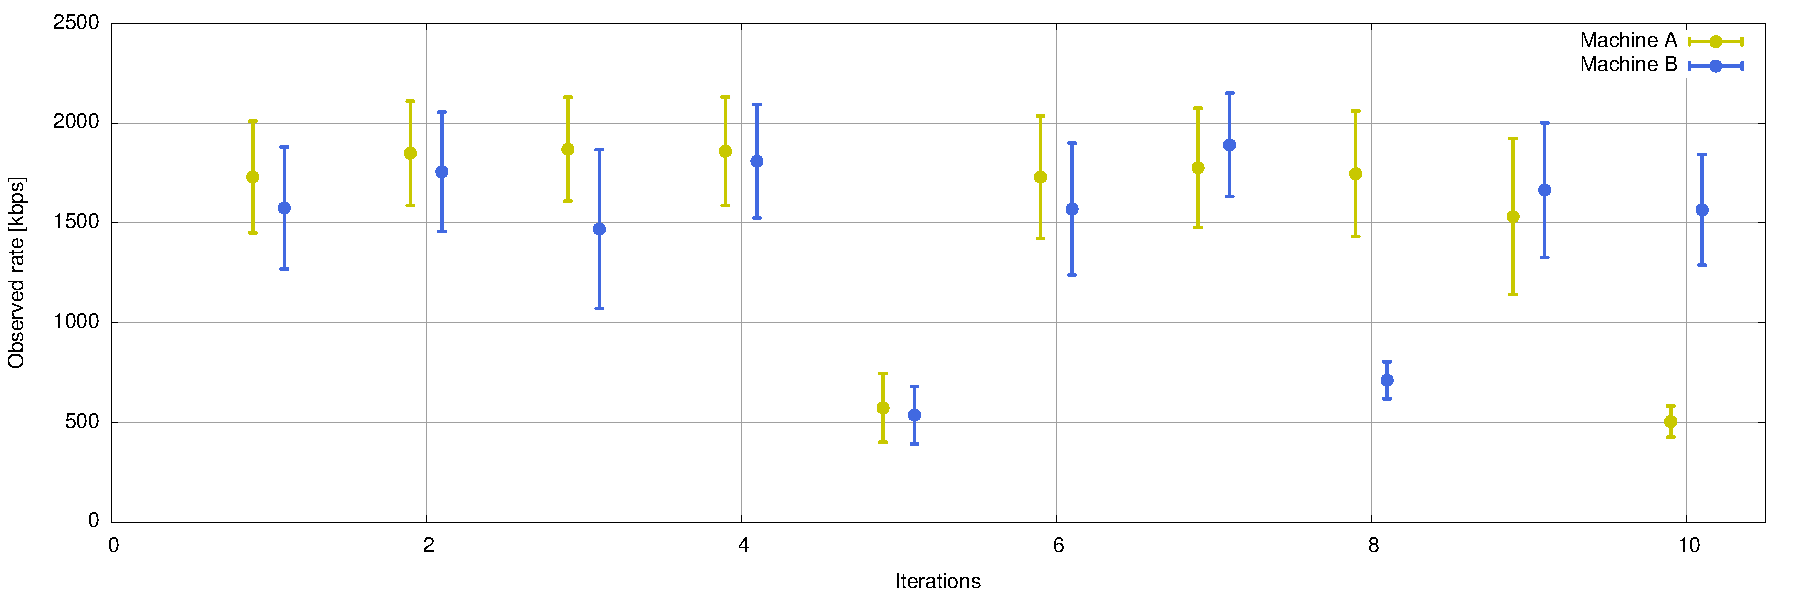
\includegraphics[width=0.75\textwidth]{100ms_bw.pdf}
  %\caption{Incoming stream}
\end{figure}
\begin{itemize}
\item 200ms
\end{itemize}
\begin{figure}[h]
  \centering
  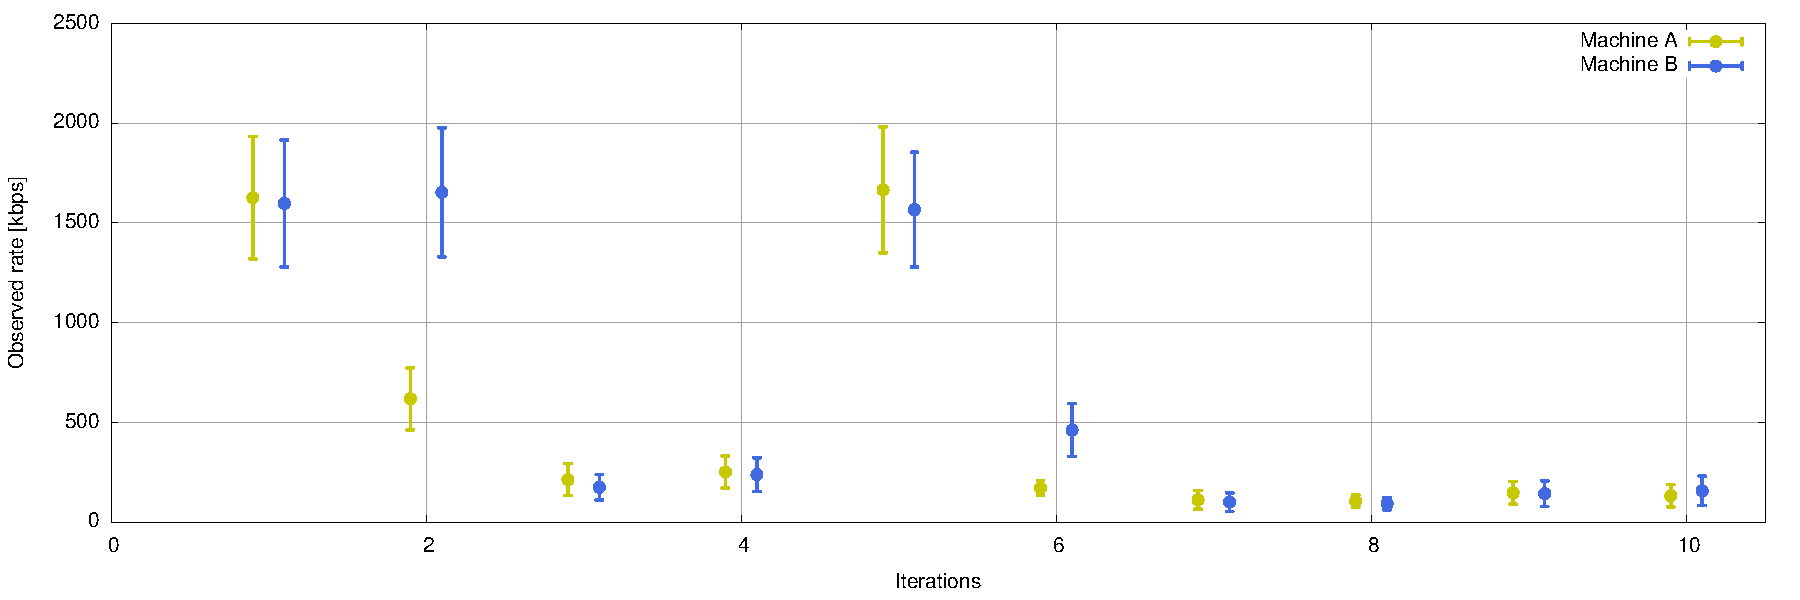
\includegraphics[width=0.75\textwidth]{200ms_bw.pdf}
  %\caption{Outgoing stream}
\end{figure}
\end{frame}

%%%%%%%%%%%%%%%%%%%%%%%%%%%%%%%%%%%%%%%%%%%%%%%%%%%%%%%%%%%%%%%%%%%%%%%%%%%%%%%%%%%%%%%%%%%%%

%\begin{frame}{Three parallel calls - topology}
%
%\begin{figure}[h]
%  \centering
%  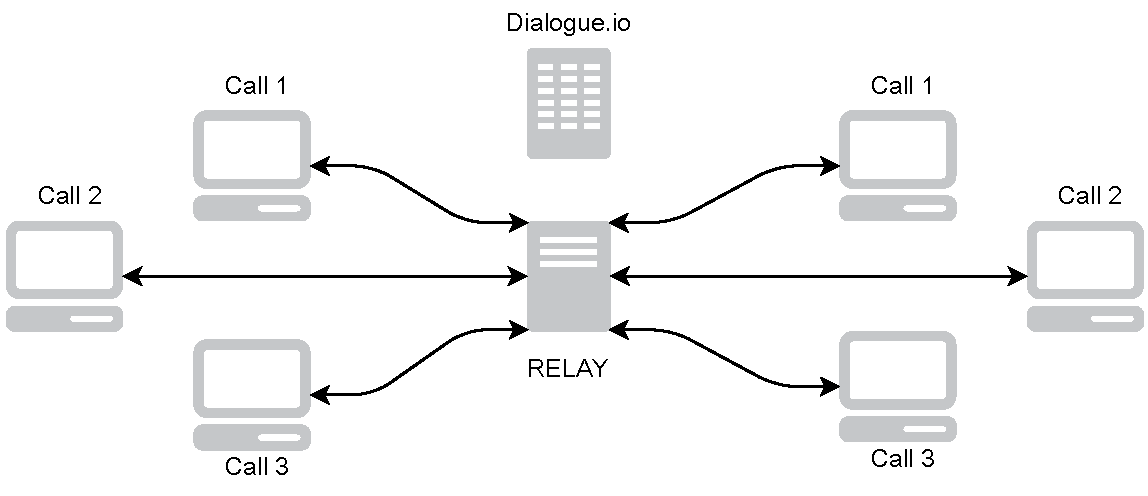
\includegraphics[width=1\textwidth]{ParallelCalls.pdf}
%\end{figure}
%
%\end{frame}

%%%%%%%%%%%%%%%%%%%%%%%%%%%%%%%%%%%%%%%%%%%%%%%%%%%%%%%%%%%%%%%%%%%%%%%%%%%%%%%%%%%%%%%%%%%%%

\begin{frame}{Three parallel calls - rate}

\begin{itemize}
\item Asynchronous
\end{itemize}
\begin{figure}[h]
  \centering
  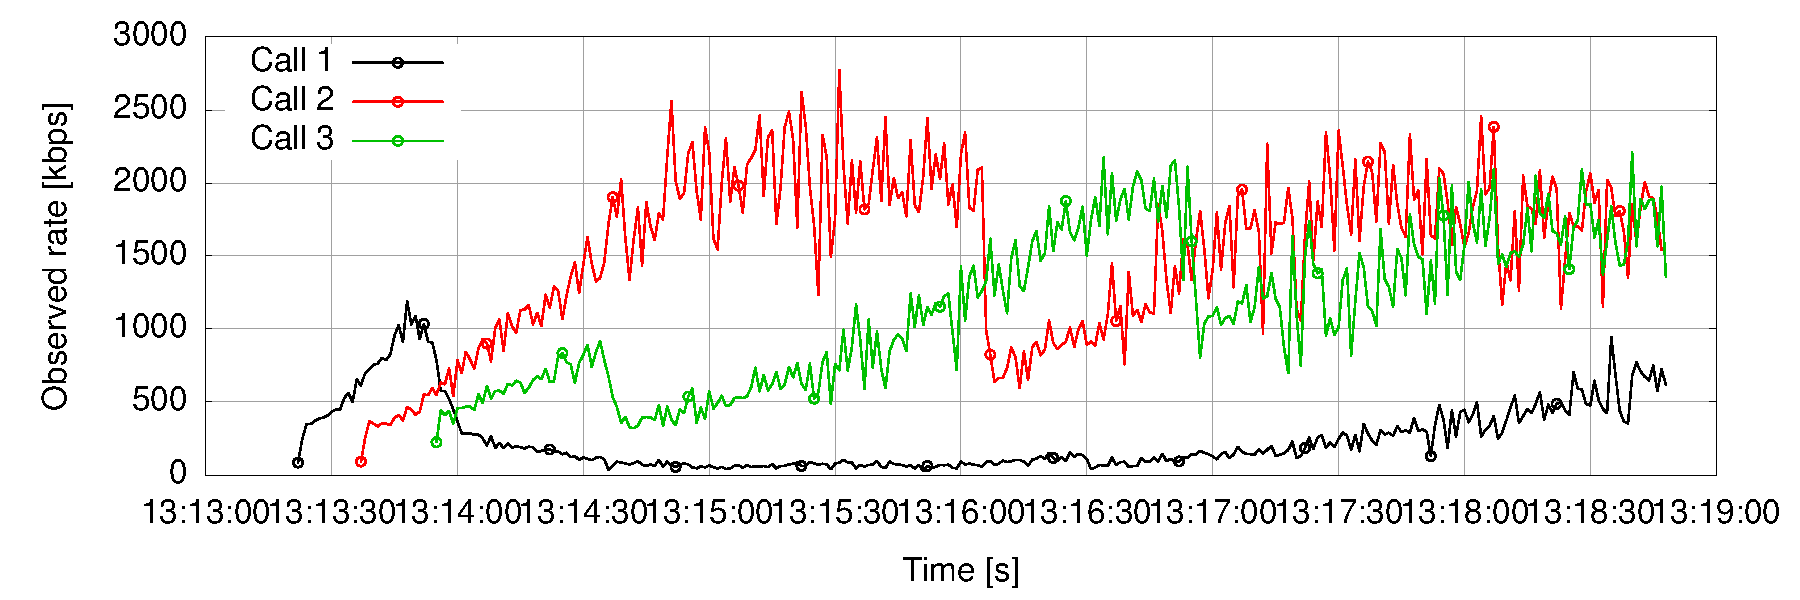
\includegraphics[width=0.75\textwidth]{async_three-calls.pdf}
  %\caption{Incoming stream}
\end{figure}
\begin{itemize}
\item Synchronous
\end{itemize}
\begin{figure}[h]
  \centering
  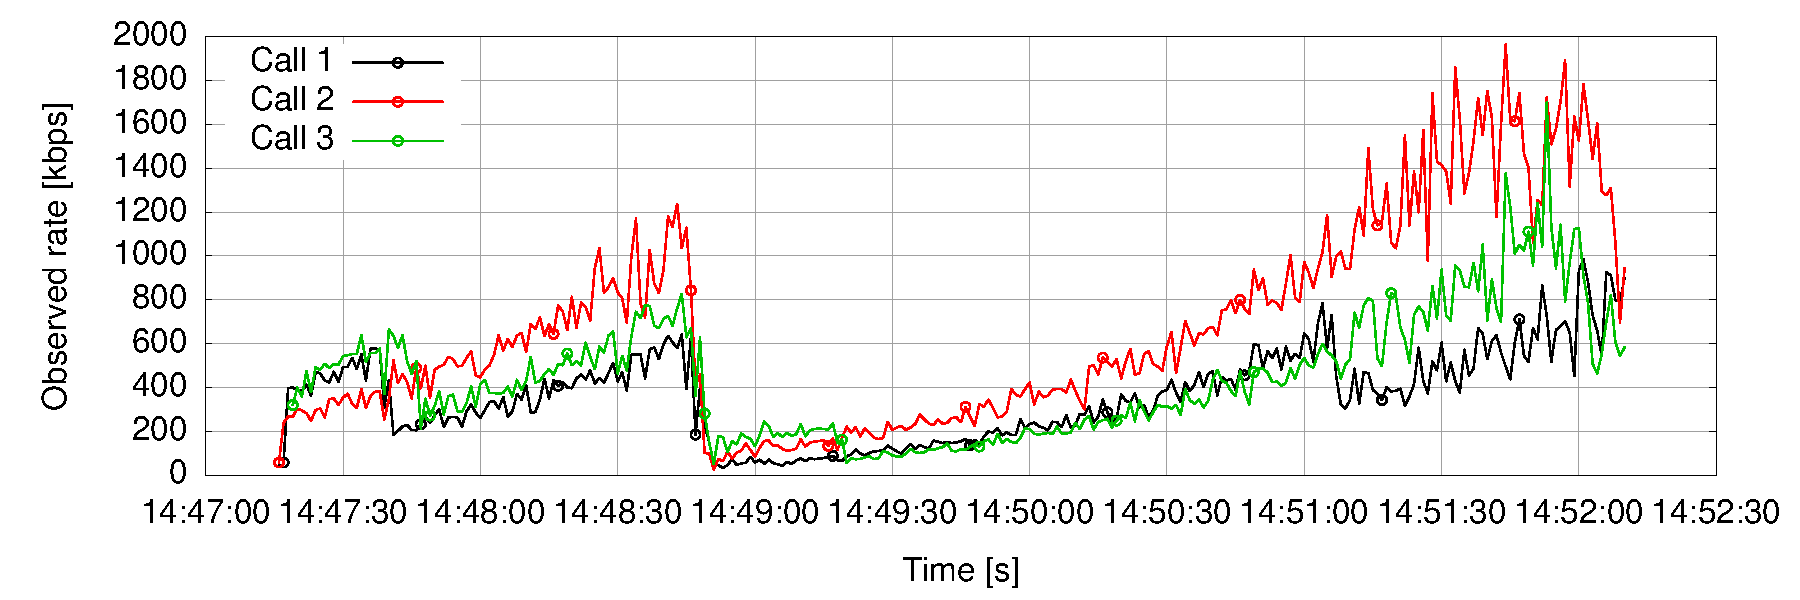
\includegraphics[width=0.75\textwidth]{sync3_three-calls20130504_195405.pdf}
  %\caption{Outgoing stream}
\end{figure}
\end{frame}

%%%%%%%%%%%%%%%%%%%%%%%%%%%%%%%%%%%%%%%%%%%%%%%%%%%%%%%%%%%%%%%%%%%%%%%%%%%%%%%%%%%%%%%%%%%%%

\begin{frame}{Three parallel calls - delay}

\begin{itemize}
\item Asynchronous
\end{itemize}
\begin{figure}[h]
  \centering
  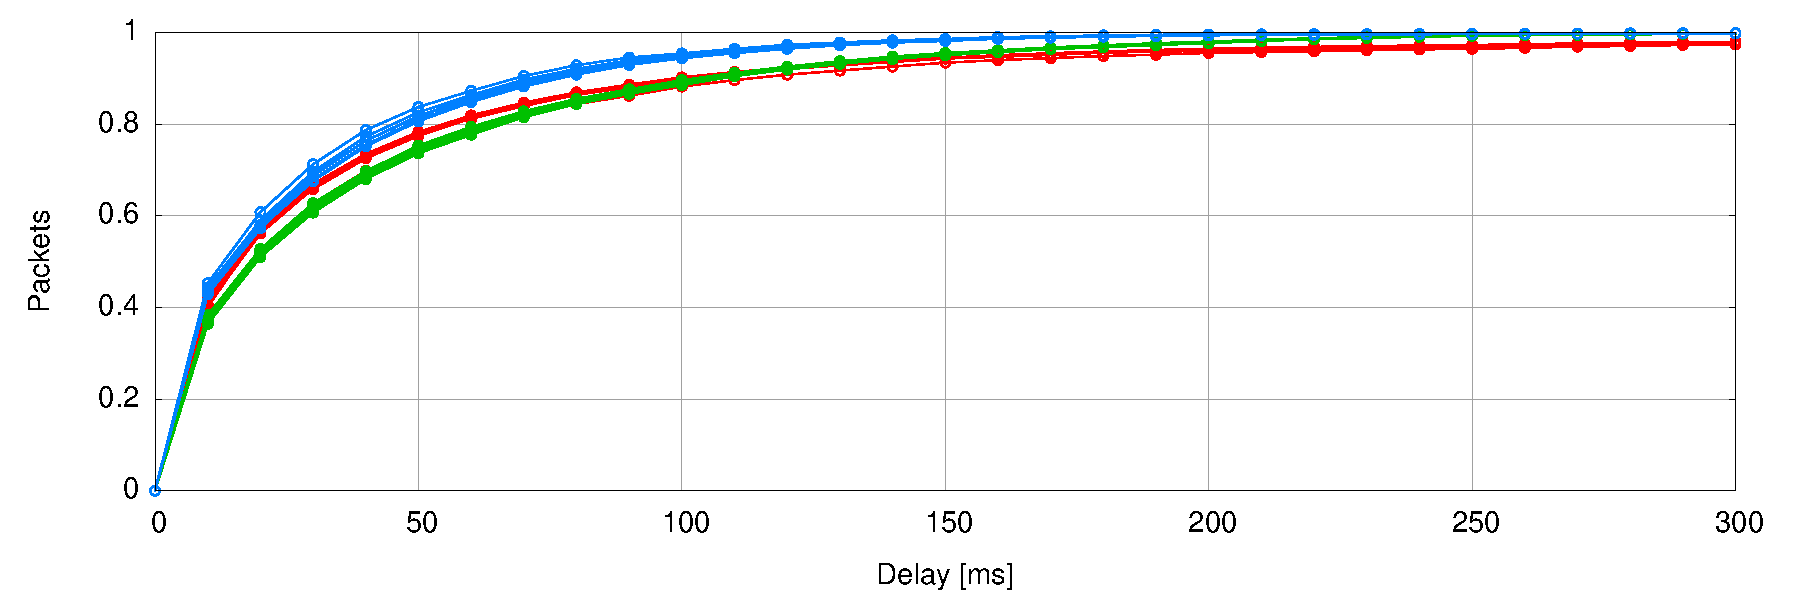
\includegraphics[width=0.75\textwidth]{async_total_delay_distribution.pdf}
  %\caption{Incoming stream}
\end{figure}
\begin{itemize}
\item Synchronous
\end{itemize}
\begin{figure}[h]
  \centering
  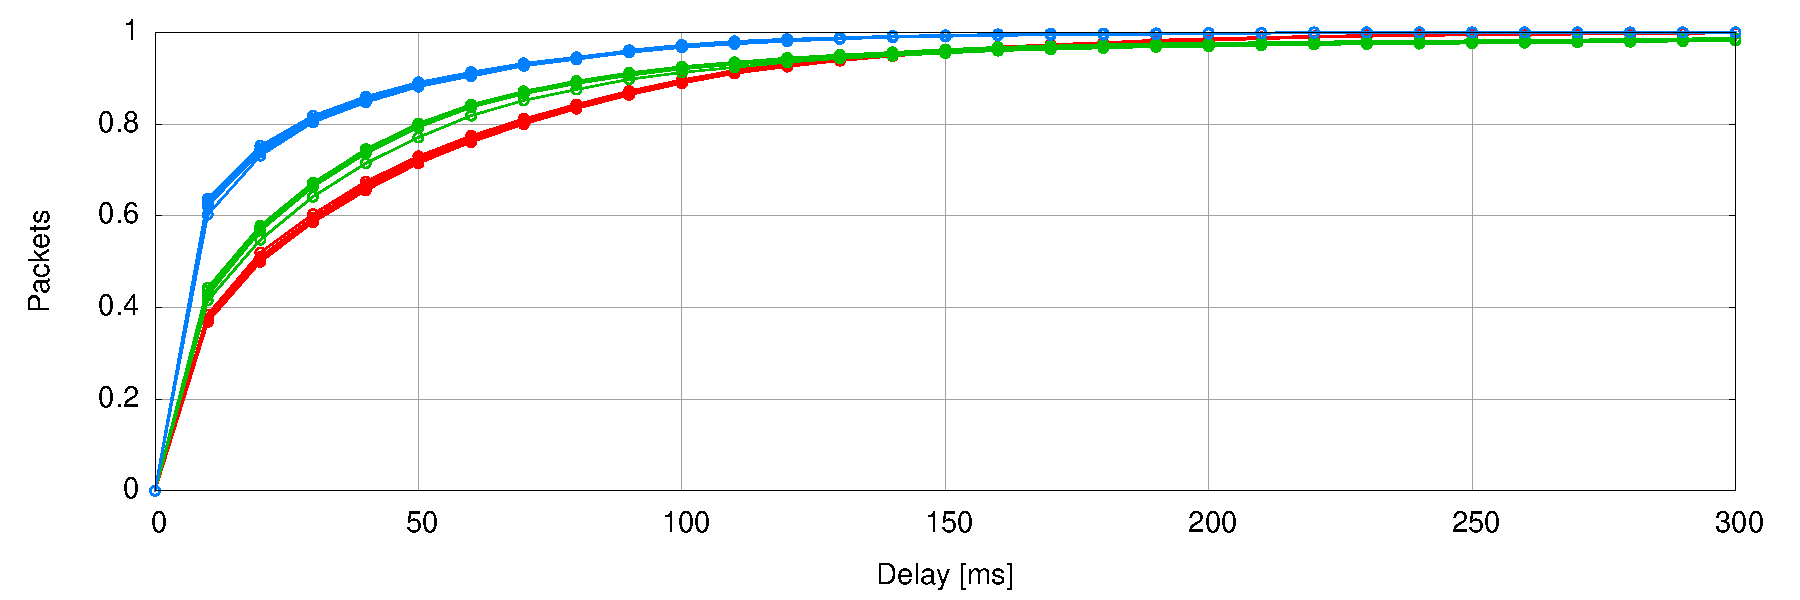
\includegraphics[width=0.75\textwidth]{three_parallel_total_delay_distribution.pdf}
  %\caption{Outgoing stream}
\end{figure}
\end{frame}

%%%%%%%%%%%%%%%%%%%%%%%%%%%%%%%%%%%%%%%%%%%%%%%%%%%%%%%%%%%%%%%%%%%%%%%%%%%%%%%%%%%%%%%%%%%%%

\begin{frame}{Interoperability}

This test evaluates the congestion mechanisms between {\it Chrome} and {\it Firefox}. 
\begin{figure}[h]
  \centering
  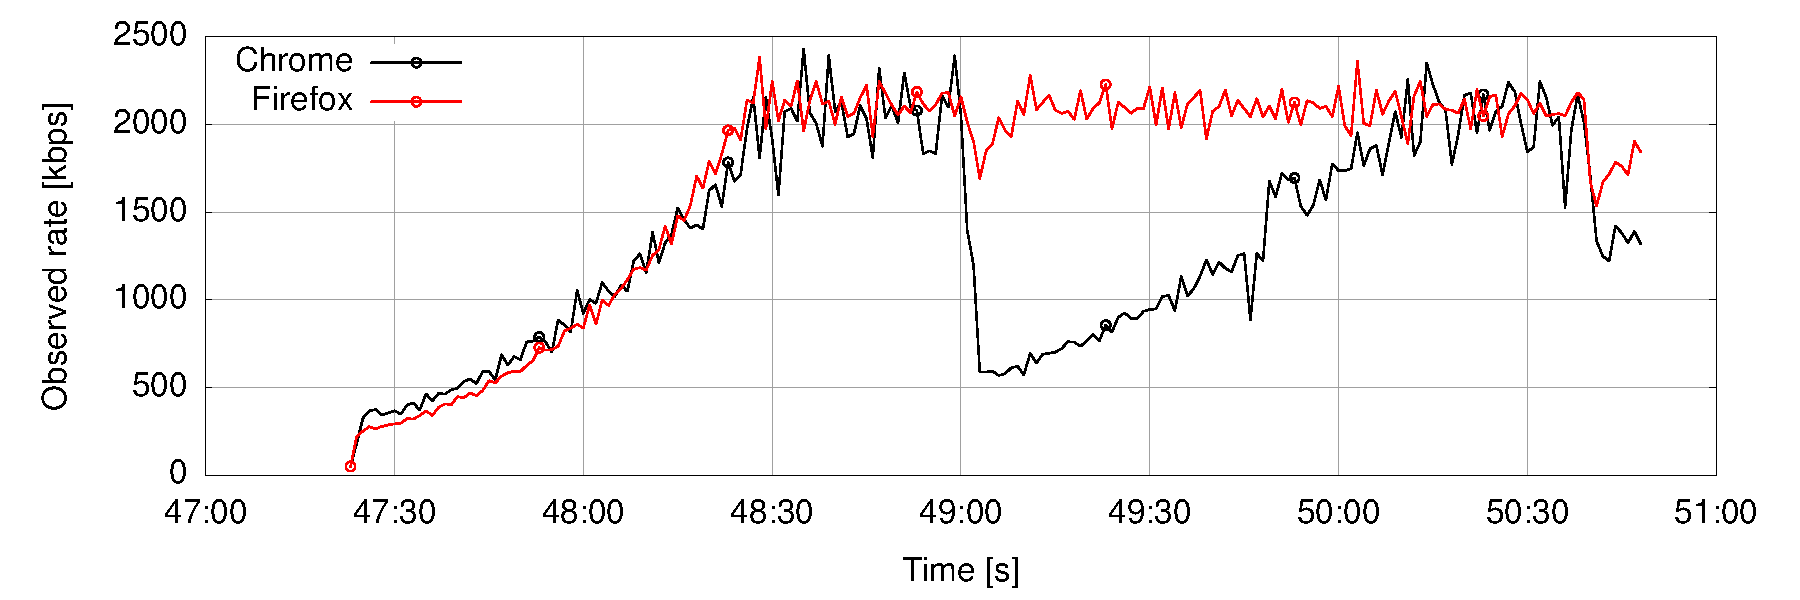
\includegraphics[width=1\textwidth]{firefoxvschrome1.pdf}
\end{figure}
{\it Firefox} is not running any congestion mechanisms to adapt the rate based on the RTCP feedback, thus is only sending Receiver Reports to the sender.
\end{frame}

%%%%%%%%%%%%%%%%%%%%%%%%%%%%%%%%%%%%%%%%%%%%%%%%%%%%%%%%%%%%%%%%%%%%%%%%%%%%%%%%%%%%%%%%%%%%%
\begin{frame}{Conclusion}

\begin{itemize}
\item Congestion mechanisms have very bad response in delayed networks
\item Interoperability cannot be achieved for low latency scenarios until {\it Firefox} enables all congestion mechanisms 
\item WebRTC has a very bad performance in multiple {\it PeerConnection} scenario regarding CPU managment
\item Different features should be enabled in the existing APIs (overlay and media track forwarding)
\end{itemize}

\end{frame}
%%%%%%%%%%%%%%%%%%%%%%%%%%%%%%%%%%%%%%%%%%%%%%%%%%%%%%%%%%%%%%%%%%%%%%%%%%%%%%%%%%%%%%%%%%%%%
\begin{frame}{}

\centering Thank you!

\end{frame}
%%%%%%%%%%%%%%%%%%%%%%%%%%%%%%%%%%%%%%%%%%%%%%%%%%%%%%%%%%%%%%%%%%%%%%%%%%%%%%%%%%%%%%%%%%%%%


\begin{frame}{Simple Feedback Loop}

\begin{figure}[h]
  \centering
  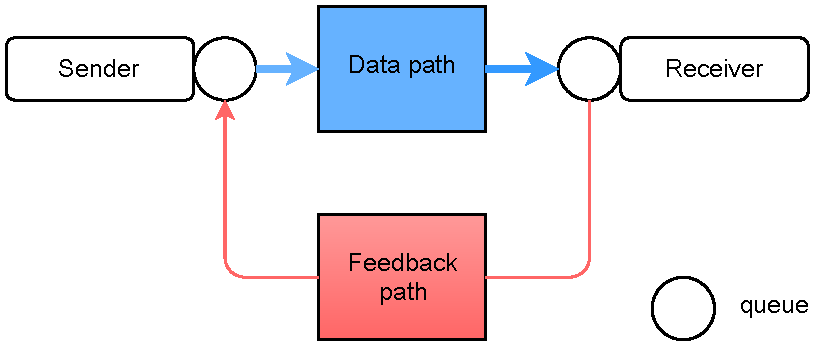
\includegraphics[width=1\textwidth]{simplefeedback.pdf}
\end{figure}
\end{frame}

%%%%%%%%%%%%%%%%%%%%%%%%%%%%%%%%%%%%%%%%%%%%%%%%%%%%%%%%%%%%%%%%%%%%%%%%%%%%%%%%%%%%%%%%%%%%%

\begin{frame}{Congestion mechanisms in WebRTC}

\begin{itemize}
\item UDP has difficulties for rate adaption 
\item Sender and Receiver RTCP reports used for rate adjustment
\item Receiver Estimated Maximum Bitrate (REMB) extension for RTCP
\item Utilizes specific {\color{red}Google algorithm} for rate adaption based on packet loss
\begin{itemize}
\item Under 2\% increases rate
\item 2-10\% reminds unchanged
\item +10\% adapts rate based on packet loss ratio
\end{itemize}
\item Rate limit by the TCP Friendly Rate Control (TFRC) formula
\end{itemize}
\end{frame}
%%%%%%%%%%%%%%%%%%%%%%%%%%%%%%%%%%%%%%%%%%%%%%%%%%%%%%%%%%%%%%%%%%%%%%%%%%%%%%%%%%%%%%%%%%%%%
\end{document}
